\documentclass[a4paper,twoside]{article}
\usepackage{jmlr2e}
\usepackage{amsmath,amssymb}
%\usepackage[T1]{fontenc}
%\usepackage[latin1]{inputenc}
%\usepackage[dvipdf]{graphicx}
\usepackage{color}
\usepackage[linesnumbered]{algorithm2e}
\usepackage[hidelinks, colorlinks=true, linkcolor=black, citecolor=blue]{hyperref} 

\newcommand{\cad}{---} % tiret cadratin
\newcommand{\gl}[1]{``\,#1\,''} % Guillemets standard
\newcommand{\ms}[1]{\texttt{#1}} %racccourci pour ``monospaced''
\newcommand{\lat}{\emph} %pour les mots latins

\newcommand{\ml}[1]{\textcolor{red}{ML : #1}}
\newcommand{\mr}[1]{\textcolor{magenta}{MR : #1}}

\jmlrheading{1}{2000}{1-48}{4/00}{10/00}{Marina Meil\u{a} and Michael I. Jordan}

\begin{document}

\title{the K-averages algorithm \\ a linear optimization alternative to kernel K-means}

\author{Mathias Rossignol \and Mathieu Lagrange}

\editor{}

\maketitle


\begin{abstract}

We present an iterative flat clustering algorithm designed to operate on arbitrary similarity matrices, with the only constraint that these matrices be symmetrical. Although functionally very close to kernel k-means, our proposal performs an maximization of average intra-class similarity, instead of a squared distance minimization, in order to remain closer to the semantics of similarities. We show that this approach allows relaxing the conditions on usable matrices, as well as opening better optimization possibilities. Systematic evaluation on a variety of data sets shows that the proposed approach outperforms or equals kernel k-means in a large majority of cases, while running much faster. Most notably, it significantly reduces memory access, which makes it a good choice for very large data collections.

\end{abstract}


\section{Introduction}

Clustering collections of objects into classes that bring together similar ones is probably the most common and intuitive tool used both by human cognition and artificial data analysis in an attempt to make that data organized, understandable, manageable. When the studied objects lend themselves to this kind of analysis, it is a powerful way to expose underlying organizations and approximate the data in such a way that the relationships between its members can be statistically understood and modeled. Given a description of objects, we first attempt to quantify which ones are ``\,similar\,'' from a given point of view, then group those $n$ objects into $C$ clusters, so that the similarity between objects within the same cluster is maximized. Finding the actual best possible partition of objects into clusters is, however, an NP-complete problem, intractable for useful data sizes, and many approaches have been proposed to yield an approximate solution: analytic, iterative, flat or hierarchical, agglomerative or divisive, soft or hard clustering algorithms, \textit{etc.}, each with their strengths and weaknesses (\cite{jain2010data}), performing better on some classes of problems than others (\cite{steinbach2000comparison,thalamuthu2006evaluation}).

Iterative divisive hard clustering algorithms, such as the ubiquitous \emph{k-means}, usually perform well to identify high-level organization in large data collections in reasonable running time; their main drawback being that the number of desired clusters must be specified. For that reason, they are a sensible choice in many data mining situations, and constitute our focus in this paper.

If the data lies in a vector space, \textit{i.e.} an object can be described by a $m$-dimensional feature vector without significant loss of information, the seminal \emph{K-means} algorithm (\cite{macQueenBsmsp67}) is probably the most efficient approach, since the explicit computation of the cluster centroids ensure both computational efficiency and scalability. This algorithm is  based on the centroid model, and minimizes the intra cluster Euclidiean distance. As shown by \cite{Banerjee:2005:CBD:1046920.1194902}, any kind of Bregman divergence, such as the KL-divergence (\cite{Dhillon:2003:DIT:944919.944973}) or the Itakura-Saito divergence (\cite{linde:algorithm}), may also be considered to develop such efficient clustering algorithms.

However, for many types of data, the projection of a representational problem into an vector space cannot be done without significant loss of descriptive efficiency. To reduce this loss, specifically tailored measures of similarity can be considered. As a result, the input data for clustering is no longer a $n \times m$ matrix storing the $m$-dimensional vectors describing the objects, but a (usually symmetric) square matrix $S$ of size $n \times n$ which numerically encodes some sort of relationship between the objects. In this case, one has to resort to clustering algorithms based on connectivity models, since the cluster centroids cannot explicitly be computed.

Earlier attempts to solve this issue considered the k-Medoids problem, where the goal is to find the $K$ objects that maximize the average similarity with the other objects of their respective clusters, or \emph{medoids}. The Partition Around Medoids (PAM) algorithm (\cite{KaufmanRousseeuw90}) solves the k-Medoids problem but with a high complexity ($O(k(n-k)^2)i$, $n$ being the number of objects) and high number of iterations $i$, due to low convergence rate. In order to scale the approach, the Clustering LARge Applications (CLARA) algorithm (\cite{KaufmanRousseeuw90}) draws a sample of objects before running the PAM algorithm. This sampling operation is repeated several times and the most satisfying set of medoids is retained. In contrast, CLARANS (\cite{Ng:1994:EEC:645920.672827}) preserves the whole set of objects but cuts complexity by  drawing a sample of neighbors in each search for the medoids.
%, with two drawbacks: it assumes that all objects fit in main memory, and the result is sensitive to the input order \cite{Zhang:1996:BED:233269.233324}.


Following work on kernel projection (\cite{Vapnik:1995:NSL:211359}), that is, the fact that a nonlinear data transformation into some high dimensional feature space increases the probability of the linear separability of patterns within the transformed space, \cite{Girolami:2002:MKC:2325785.2326903} introduced a kernel version of the K-means algorithm, whose input is a kernel matrix $\mathcal{K}$ that must be a Gram matrix, \textit{i.e.} semi definite positive. \cite{Dhillon:2007:WGC:1313055.1313291} linked a weighted version of the kernel K-means objective to the popular spectral clustering, introducing an efficient way of solving the normalized cut objective.

The kernel K-means algorithm proved to be equally useful when considering arbitrary similarity problems if special care is taken to ensure definite positiveness of the input matrix (\cite{Roth:2003:OCP:960254.960291}). This follows original algorithmic considerations where vector space data is projected into high dimensional spaces using a carefully chosen kernel function. 

%% Long sentence! rewritten above
%Originally thought as considering data lying initially in a given vector space then projected in an high dimensional features space thanks to a carefully chosen kernel function, the kernel K-means algorithm proved to be equally useful when considering arbitrary similarity problems if some special care is taken to ensure definite positiveness of the input matrix (\cite{Roth:2003:OCP:960254.960291}).

Despite such improvements, kernel K-means can be hardly applied to large scale datasets without special treatments because of high algorithmic and memory access costs. 
%Still, the complexity of the algorithm and the cost of memory  access  prevent from using the kernel K-means algorithm for large scale datasets without specific treatments. 
\cite{Chitta:2011:AKK:2020408.2020558} considered sampling of the input data, \cite{1047453} considered block storing of the input matrix, and a preclustering  approach (\cite{bradley98scaling, conf/icde/GantiRGPF99}) is considered by \cite{Kulis2008} with a coarsening and refining phases as respectively a pre- and post-treatment of the actual clustering phase.

The work we present is this paper results from an effort to directly maximize the average intra-class similarity, without resorting to a geometric interpretation of data. Following that idea allows us to propose a new hard clustering algorithm, which we call \emph{k-averages}, with the following properties: 
\begin{itemize}
%\item it may consider as input arbitrary symmetric similarity matrices,
\item input data can be arbitrary symmetric similarity matrices,
\item it has fast and guaranteed convergence, with a low number of object to clusters reallocations,
\item it provides good scalability thanks to a reduced need for memory access, and
\item on a collection of synthetic and natural test data, its results are on average slightly better than those of kernel k-means, and obtained in a fraction of its computing time, particularly when paged memory is required.
\end{itemize}

The remaining of the paper is organized as follows: Section~\ref{sec:kkmeans} presents the kernel K-means objective function and the basic algorithm that minimizes this function, and Section~\ref{sec:kaverages} introduces the concepts behind the k-averages algorithm, 
%before giving a detailed description of it in Section~\ref{sec:algo}. 
followed by a detailed algorithmic description in Section~\ref{sec:algo}. 
The complexity of the two algorithms in terms of arithmetic operations and memory access is then studied in Section \ref{sec:complexity}. The above presented properties of the proposed k-averages algorithm are then validated on synthetic controlled data in Section \ref{sec:validation} and on 43 corpora of time series in Section \ref{sec:experiments}.

\section{kernel K-means} \label{sec:kkmeans}

Since its introduction by \cite{Girolami:2002:MKC:2325785.2326903}, kernel k-means has been an algorithm of choice for flat data clustering with known number of clusters (cite salient uses of kkmeans). It makes use of a mathematical technique known as the \gl{kernel trick} to extend the classical k-means clustering algorithm (\cite{macQueenBsmsp67}) to criteria beyond simple euclidean distance proximity. Since it constitutes the closest point of comparison with our own work, we dedicate this section to its detailed presentation.

In the case of kernel k-means, the kernel trick consists in considering that the k-means algorithm is operating in an unspecified, possibly very high-dimensional Euclidian space; but instead of specifying the properties of that space and the coordinates of objects, the equations governing the algorithm are modified so that everything can be computed knowing only the scalar products between points. The symmetrical matrix  containing those scalar products is known as a kernel, noted $\mathcal{K}$.

\subsection{Kernel k-means objective function}

In this section and the following, we shall adopt the following convention: $N$ is the number of objects to cluster and $C$ the number of clusters; $N_c$ is the number of objects in cluster $c$, and $\mu_c$ is the centroid of that cluster. $z_{cn}$ is the membership function, whose value is $1$ if object $o_n$ is in class $c$, $0$ otherwise.

Starting from the objective function minimized by the k-means algorithm, expressing the sum of squared distances of points to the centroids of their respective clusters:

\[
S = \sum_{c=1}^{C} \sum_{n=1}^{N} z_{cn} \left(o_n-\mu_c\right)\left(o_n-\mu_c\right)^\top \label{eq:S}
\]

And using the definition of centroids as:

\[
\mu_c = \frac{1}{N_c}\sum_{n=1}^{N}z_{cn}o_n
\]

$S$ can be developed and rewritten in a way that does not explicitly refer to the centroid positions, since those cannot be computed:

\[
S = \sum_{c=1}^{C} \sum_{n=1}^{N} z_{cn} Y_{cn}
\]

where
\begin{eqnarray}
Y_{cn} & = & \left(o_n-\mu_c\right)\left(o_n-\mu_c\right)^\top \\
       & = & o_n.o_n - 2 o_n.\mu_c + \mu_c.\mu_c \\
       & = & o_n.o_n - 2 o_n.\frac{1}{N_c} \sum_{i=1}^{N} z_{ci} o_i +
       	 \left(\frac{1}{N_c} \sum_{i=1}^{N} z_{ci} o_i\right).\left(\frac{1}{N_c} \sum_{i=1}^{N} z_{ci} o_i\right) \\
       & = & o_n.o_n - \frac{2}{N_c} \sum_{i=1}^{N} z_{ci} o_n.o_i +
       	 \frac{1}{N_c^2} \sum_{i=1}^{N} \sum_{j=1}^{N} z_{ki} z_{kj} o_i.o_j \\
       & = & \mathcal{K}_{nn} - \frac{2}{N_c} \sum_{i=1}^{N} z_{ci} \mathcal{K}_{ni} +
         \frac{1}{N_c^2} \sum_{i=1}^{N} \sum_{j=1}^{N} z_{ki} z_{kj} \mathcal{K}_{ij} \label{eq:yki}
\end{eqnarray}

%% Comment by Arshia: The following paragraph is too fast!
% what does "mostly bounded" mean?
% The second half going to "similarity matrix processing" can be further explained.. this means that K_nn will become similarity measures.. right?

Since the sum of $K_{nn}$ over all points remains constant, and the sum of squared centroid norms (third, quadratic, term of Equation~\ref{eq:yki}) is mostly bounded by the general geometry of the cloud of objects, we can see that minimizing this value implies maximizing the sum of the central terms, which are the average scalar products of points with other points belonging to the same class. Given a similarity matrix possessing the necessary properties to be considered as a kernel matrix (positive semidefinite), the kernel k-means algorithm can therefore be used to create clusters that somehow maximize the average intra-cluster similarity.

\subsection{Algorithm}

Finding the configuration that absolutely minimizes S (eq~\ref{eq:S}) is an NP-complete problem. However, several approaches allow finding a good approximate result. We shall only focus here on the fastest and most popular, an iterative assignment\,/\,update procedure commonly referred to as the \gl{k-means algorithm} (\cite{macQueenBsmsp67}), or as a discrete version of Lloyd's algorithm, detailed in Algorithm~\ref{algo:kkmeans}.
% Arshia: Cite algorithm source? MR: yes, added

\begin{algorithm}
	\label{algo:kkmeans}
	\SetAlgoLined
	\KwData{number of objects $N$, number of classes $C$, kernel matrix $\mathcal{K}$}
	\KwResult{label vector $L$ defining a partition of the objects into $C$ classes}
	\BlankLine	
	\textbf{Initialization:} fill L with random values in $[1..C]$\;
	\BlankLine	
	\While {$L$ is modified} {
		\For {$n \leftarrow 1$ to $N$} {
			\For {$c \leftarrow 1$ to $C$} {
				Compute $Y_{cn}$ following eq~\ref{eq:yki} \label{algline:kkmeans_cplx1}
				(note: $z_{cn} = (L_n == c)\,?\,1\;:\;0$)
			}
			$L_n = \textrm{argmin}_c (Y_{cn})$\;
		}
	}
	\BlankLine
	\caption{Lloyd's algorithm applied to minimizing the kernel k-means objective.}
\end{algorithm}

The version given here is the most direct algorithmic translation of the mathematical foundations developed above, and as we shall see in section~\ref{sec:complexity}, it can easily become more efficient. Before that, we introduce our proposed k-averages algorithm.


\section{Foundations of the k-averages algorithm} \label{sec:kaverages}

In our proposal, we adopt an alternative objective function which, unlike kernel k-means, does not rely on a geometric interpretation but an explicit account of the similarity matrix. The goal is to maximize the average intra-cluster similarity between points, a commonly used metric to evaluate clustering quality, and one whose computation is very direct\cad{}linear in time.

Due to its simplicity, however, the objective function cannot be simply "plugged into" the standard kernel k-means algorithm: it lacks the geometric requisites to ensure convergence. We must therefore propose an adapted algorithmic framework to exploit it: first, we show here that it is possible to easily compute the impact on the global objective function of moving a single point from one class to another; we then introduce an algorithm intended to take advantage of that formula.

\subsection{Conventions and possible objective functions}

In addition to the notations already presented above, we index here the set of elements belonging to a given cluster $c_k$ as $c_k = \left\{o_{k1}, \ldots, o_{kN_k}\right\}$. 
For simplicity, we omit the first index and note $c = \left\{o_1, \ldots, o_{N_c}\right\}$ when considering a single class. 
%To simplify below, when we're simply considering one class, no matter
%which, we shall omit the first index and write $c = \left\{o_1, \ldots, o_{N_c}\right\}$.

The similarity between objects shall be written $s\left(o_i, o_j\right)$.
%Let us 
We extend the notation $s$ to the \emph{similarity of an object to a
  class} defined as the average similarity of an object
with all objects of the class. $s(o,c)$ accepts two definitions,
depending on whether or not $o$ is in $c$:

If $o \notin c$,
\begin{equation}
  s\left(o,c\right) = \frac{1}{N_c} \sum_{i=1}^{n_c}s\left(o, o_i\right)
   \label{eq:soc_notinclass}
\end{equation}

If $o \in c$, then necessarily $\exists i \mid o = o_i$
\begin{equation}
  s\left(o,c\right) = s\left(o_i, c\right) = \frac{1}{N_c-1} \sum_{j=1 \ldots n_c, j \neq i} s\left(o_i, o_j\right)
  	 \label{eq:soc_inclass}
\end{equation}

Let's call \gl{quality} of a class the average intra-class object-to-object similarity, and write it $\mathcal{Q}$:
\begin{equation}
\mathcal{Q}\left(c\right) = \frac{1}{N_c} \sum_{i=1}^{n_c} s\left(o_i, c\right)
\end{equation}

In our framework, we do not explicitly refer to class centroids, preferring to directly consider averages of similarity values between individuals within clusters. Indeed, we never refer to a geometrical interpretation of the data. However, it should be noted that since in k-means (and kernel k-means) the centroid of a class is defined as an average of all points in that class, $\mathcal{Q}$ is strictly equivalent to the average point to centroid similarity.

Using the notations above, we define our objective function as the average class quality, %normalized taking into account the class sizes:
normalized with class sizes:

\[
O_2 = \frac{1}{N} \sum_{i=1}^{C} N_i \mathcal{Q}(c_i)
\]

Since informally, our goal is to bring together objects that share high similarity, a first idea would be to simply move each object to the class with whose members it has the highest average similarity. This is what we call the \gl{naive k-averages} algorithm.

\subsection{Naive k-averages algorithm}

Algorithm~\ref{algo:naive-kaverages} presents a method that simply moves each object to the class with which it has the highest average similarity, until convergence is reached. The algorithm is straightforward and simple; however, experiments show that while it can often produce interesting results, it also sometimes cannot reach convergence because the decision to move an object to a different cluster is taken without considering the impact of the move on the quality of the source cluster.

\begin{algorithm}
	\label{algo:naive-kaverages}
	\SetAlgoLined
	\KwData{number of objects $N$, number of classes $C$, kernel matrix $\mathcal{K}$}
	\KwResult{label vector $L$ defining a partition of the objects into $C$ classes}
	\BlankLine	
	\textbf{Initialization:} 
		Fill L with random values in $[1..C]$\;
		Compute initial object-class similarities $S$ following eq~\ref{eq:soc_inclass} or eq~\ref{eq:soc_notinclass}\;
	\BlankLine	
	\While {$L$ is modified} {
		\For {$i \leftarrow 1$ to $N$} {
			previousClass $\leftarrow L_i$\;
			nextClass $\leftarrow \mathrm{argmin}_k\, S(i, k)$
			\If {nextClass $\ne$ previousClass} {
				$L_i \leftarrow \mathrm{nextClass}$\;
				\For {$j \leftarrow 1$ to $N$}{
					Update $S(j,nextClass)$ and $S(j,previousClass)$
				}
			}
		}
	}
	\BlankLine
	\caption{Naive k-averages algorithm.}
\end{algorithm}

To ensure global convergence, we need to compute the impact on the global objective function of moving one object from one class to another. Using such formulation and performing only reallocation that have a positive impact, we shall then be in position to guarantee the convergence of an iterative algorithm. 

\subsection{Impact of object reallocation on class quality}

Considering a class $c$, let us develop the expression of $\mathcal{Q}(c)$ into a more useful form. Since all objects are in $c$, we use the formula in (\ref{eq:soc_inclass}) to get:

\begin{equation}
  \begin{aligned}
    \mathcal{Q}\left(c\right) & = \frac{1}{N_c} \sum_{i=1}^{N_c} \frac{1}{N_c-1} \sum_{\substack{j=1 \ldots N_c\\j \neq i}} s\left(o_i, o_j\right) \\
                              & = \frac{1}{N_c(N_c-1)} \sum_{i=1}^{N_c} \sum_{\substack{j=1 \ldots N_c\\j \neq i}} s\left(o_i, o_j\right)
  \end{aligned}
\end{equation}

Using the assumption that the similarity matrix is symmetrical, we can reach: % (this is an indispensable transformation for future calculations):
\begin{equation}
    \mathcal{Q}\left(c\right) = \frac{2}{N_c(N_c-1)} \sum_{i=2}^{N_c} \sum_{j=1}^{i-1} s\left(o_i, o_j\right)
    \label{eq:classQuality}
\end{equation}

For future use and given the importance of the above transformation, we define:
\begin{equation}
  \Sigma(c) = \sum_{i=2}^{N_c} \sum_{j=1}^{i-1} s\left(o_i, o_j\right)
\end{equation}

Thus:
\begin{equation}
    \mathcal{Q}\left(c\right) = \frac{2}{N_c(N_c-1)}\Sigma(c) \phantom{XX}\mathrm{and}\phantom{XX} \Sigma(c) = \frac{N_c(N_c-1)\mathcal{Q}\left(c\right)}{2}
\end{equation}


\subsubsection{Removing an object from a class}

Assuming that $o \in c$, necessarily $\exists i \mid o=o_i$. Since the numbering of objects is arbitrary, we can first simplify the following equation by considering that $o = o_{N_c}$, in order to reach a formula that is independent from that numbering.

% Arshia: Above sentence is not clear "then generalise"?

\begin{equation}
  \begin{aligned}
    \mathcal{Q}\left(c \smallsetminus o_{N_c}\right) & = \frac{2}{(N_c-1)(N_c-2)} \sum_{i=2}^{N_c-1} \sum_{j=1}^{i-1} s\left(o_i, o_j\right) \\
                                                   & = \frac{2}{(N_c-1)(N_c-2)} \left[\Sigma(c) - \sum_{j=1}^{N_c-1} s\left(o_{N_c}, o_j\right) \right] \\
                                                   & = \frac{2}{(N_c-1)(N_c-2)} \left[\Sigma(c) - (N_c-1)s\left(o_{N_c}, c\right) \right] \\
                                                   & = \frac{2N_c(N_c-1)\mathcal{Q}(c)}{2(N_c-1)(N_c-2)} - \frac{2(N_c-1)s\left(o_{N_c}, c\right)}{(N_c-1)(N_c-2)}\\
                                                   & = \frac{N_c \mathcal{Q}(c)  - 2s\left(o_{N_c}, c\right)}{N_c-2}
  \end{aligned}
\end{equation}

The quality of a class after removal of an object is thus:

\begin{equation}
  \mathcal{Q}\left(c \smallsetminus o\right) = \frac{N_c \mathcal{Q}(c)  - 2s\left(o, c\right)}{N_c-2}
  \label{eq:newQual_remove}
\end{equation}

And the change in quality from its previous value:

\begin{equation} \label{deltaRemove}
  \begin{aligned}
    \mathcal{Q}\left(c \smallsetminus o\right) - \mathcal{Q}\left(c\right) & = \frac{N_c \mathcal{Q}(c)  - (N_c-2) \mathcal{Q}(c)  - 2s\left(o, c\right)}{N_c-2} \\
                                                                           & = \frac{2\left( \mathcal{Q}(c) - s\left(o, c\right)\right)}{N_c-2}
    \end{aligned}
\end{equation}


\subsubsection{Adding an object to a class}

Assuming that $o \notin c$, we can similarly to what has been done previously (numbering is arbitrary) consider for the sake of simplicity that $o$ becomes $o_{N_c+1}$ in the modified class $c$. Following a path similar to above, we get:

\begin{equation}
  \begin{aligned}
    \mathcal{Q}(c \cup o_{N_c+1}) & = \frac{2}{N_c(N_c+1)} \sum_{i=2}^{N_c+1} \sum_{j=1}^{i-1} s\left(o_i, o_j\right) \\
                                & = \frac{2}{N_c(N_c+1)} \left[\Sigma(c) + N_c s\left(o_{N_c+1}, c\right)\right] \\
                                & = \frac{(N_c-1) \mathcal{Q}(c)  + 2s\left(o_{N_c+1}, c\right)}{N_c+1}
  \end{aligned}
\end{equation}

\noindent The quality of a class $c$ after adding an object $o$ is thus:

\begin{equation}
  \mathcal{Q}\left(c \cup o\right) = \frac{(N_c-1) \mathcal{Q}(c)  + 2s\left(o, c\right)}{N_c+1}
  \label{eq:newQual_add}
\end{equation}

\noindent And the change in quality from its previous value:

\begin{equation} \label{deltaAdd}
  \begin{aligned}
    \mathcal{Q}\left(c \cup o\right) - \mathcal{Q}\left(c\right) & = \frac{(N_c-1) \mathcal{Q}(c)  - (N_c+1) \mathcal{Q}(c)  + 2s\left(o, c\right)}{N_c+1} \\
                                                                           & = \frac{2\left(s\left(o, c\right)-\mathcal{Q}(c)\right)}{N_c+1}
    \end{aligned}
\end{equation}


\subsection{Impact of object reallocation on the global objective function}

When moving an object $o$ from class $c_s$ (\gl{source}), to whom it belongs, to a
distinct class $c_t$ (\gl{target}), $(N_s-1)$ objects are affected
by the variation in (\ref{deltaRemove}), and $N_t$ are affected
by that in (\ref{deltaAdd}); in addition, one object $o$ moves from a class whose quality is $\mathcal{Q}(c_s)$ to one whose quality is $\mathcal{Q}\left(c_t \cup o\right)$, as expressed by equation~\ref{eq:newQual_add}:

\begin{equation}
  \delta_o(c_s, c_t) = \frac{2N_t \left(s\left(o, c_t\right)-\mathcal{Q}(c_t)\right)}{N_t+1} + \frac{2(N_s-1)\left( \mathcal{Q}(c_s) - s\left(o, c_s\right)\right)}{N_s-2} - \mathcal{Q}(c_s) + \frac{(N_t-1) \mathcal{Q}(c_t)  + 2s\left(o, c_t\right)}{N_t+1}
  \label{eq:impact_classnorm}
\end{equation}

As can be seen, computing this impact is a fixed-cost operation. We can therefore use the formula as the basis for an efficient iterative algorithm.

\section{K-averages algorithm}
\label{sec:algo}

Our approach does not allow us to benefit, like kernel k-means, from the convergence guarantee brought by the geometric foundation of k-means. In consequence, we cannot apply a \gl{batch} approach where at each iteration all elements are moved to their new class, and all distances (or similarities) are computed at once. Therefore, for each considered object, after finding its ideal new class, we must update the class properties for the two modified classes (source and destination), as well as recompute the average class-object similarities for them.

At a first glance, dynamically updating objectives as a result of object reallocation might seem to have negative performance impact. However, our simple non-quadratic updates makes such dynamic changes easily tractable. New class qualities are thus given by Equations~\ref{eq:newQual_remove} and \ref{eq:newQual_add}, and new object-class similarities can be computed by:

%% Rewritten above.. feel free to modify!!! (Arshia)
%Although this seems at first like systematically updating everything at each object re-allocation should have a huge performance impact, our reliance on simple averages without any quadratic terms makes it possible to have very simple update formulas: new class qualities are given by Equations~\ref{eq:newQual_remove} and \ref{eq:newQual_add}, and new object-class similarities can be computed by:

\begin{equation}
	\begin{aligned}
    s(i, c_s(t+1)) &= \frac{N_s(t).s(i, c_s(t)) + s(i,n)}{N_s(t)+1} \\
    s(i, c_t(t+1)) &= \frac{N_t(t).s(i, c_s(t)) - s(i,n)}{N_t(t)-1}
   	\end{aligned}
  \label{eq:newSimilNewC}
\end{equation}

\noindent where $i$ is any object index, $n$ is the recently reallocated object, $c_s$ the \gl{source} class that object $i$ was removed from, and $c_t$ the \gl{target} class that object $n$ was added to.

The full description of k-averages is given in Algorithm~\ref{algo:kaverages}.

\begin{algorithm}
	\label{algo:kaverages}
	\SetAlgoLined
	\KwData{number of objects $N$, number of classes $C$, similarity matrix $\mathcal{S}$}
	\KwResult{label vector $L$ defining a partition of the objects into $C$ classes}
	\BlankLine	
	\textbf{Initialization:}
		Fill L with random values in $[1..C]$\;
		Compute initial object-class similarities $S$ following eq~\ref{eq:soc_inclass} or eq~\ref{eq:soc_notinclass}\;
		Compute initial class qualities $\mathcal{Q}$ following eq~\ref{eq:classQuality}\;
	\BlankLine	
	\While {$L$ is modified} {
		\For {$i \leftarrow 1$ to $N$} {
			previousClass $\leftarrow L_i$\;
			nextClass $\leftarrow \mathrm{argmin}_k\,\delta_i(\mathrm{previousClass}, k)$ \label{algline:kaverages_search}
			(following the definition of $\delta$ in eq~\ref{eq:impact_objnorm} or \ref{eq:impact_classnorm})\;
			\If {nextClass $\ne$ previousClass} {
				$L_i \leftarrow \mathrm{nextClass}$\;
				Update $\mathcal{Q}_\mathrm{previousClass}$ following eq~\ref{eq:newQual_remove}\;
				Update $\mathcal{Q}_\mathrm{nextClass}$ following eq~\ref{eq:newQual_add}\;
				\For {$j \leftarrow 1$ to $N$}{
					Update $S(j,nextClass)$ and $S(j,previousClass)$ \label{algline:kaverages_recompute} \\ following eq~\ref{eq:newSimilNewC}\;
				}
			}
		}
	}
	\BlankLine
	\caption{K-averages algorithm.}
\end{algorithm}


\section{Complexity analysis}
\label{sec:complexity}

In this section, we study the complexity of the two approaches presented above, first form the point of view of raw complexity, then focusing on memory access.

\subsection{Computational complexity}

\subsubsection{Kernel k-means}

As can be seen in Algorithm~\ref{algo:kkmeans}, the operation on line~\ref{algline:kkmeans_cplx1} is the most costly part of the algorithm: for each object $n$ and class $c$, at each iteration, it is necessary to compute $Y_{cn}$ from Equation~\ref{eq:yki}\cad{}an $O(N^2)$ operation in itself, per object. The impossibility of simply computing the distances to a known centroid as is done in simple k-means gives kernel k-means a much higher complexity, globally $O(N^3)$ per iteration, independent of how many objects are moved for that iteration.

It is however possible to improve the performance of kernel k-means by noting than in Equation~\ref{eq:yki}, the third term of the equation, which has the highest complexity, is only dependent on class definitions and not on the considered object. We can therefore rewrite Equation~\ref{eq:yki} as:

\begin{eqnarray}
Y_{cn} & = & \mathcal{K}_{nn} - \frac{2}{N_c} \sum_{i=1}^{N} z_{ci} \mathcal{K}_{ni} + M_c \label{eq:yki_improved}
\end{eqnarray}
where
\begin{eqnarray}
M_c    & = & \frac{1}{N_c^2} \sum_{i=1}^{N} \sum_{j=1}^{N} z_{ki} z_{kj} \mathcal{K}_{ij} \label{eq:mc}
\end{eqnarray}

Algorithm~\ref{algo:kkmeans} thus becomes Algorithm~\ref{algo:kkmeans_optim}, where the values of $M_c$ are computed once at the beginning of each loop (line~\ref{algline:kkmeans_imp_mc}) then reused on line~\ref{algline:kkmeans_imp_cplx1}, thus reducing the overall complexity to $O(n^2)$ per iteration. This optimized version of kernel k-means is the one we shall consider for performance comparison in the remainder of this article.

\begin{algorithm}
	\label{algo:kkmeans_optim}
	\SetAlgoLined
	\KwData{number of objects $N$, number of classes $C$, kernel matrix $\mathcal{K}$}
	\KwResult{label vector $L$ defining a partition of the objects into $C$ classes}
	\BlankLine	
	\textbf{Initialization:}
	fill L with random values in $[1..C]$\;
	\BlankLine	
	\While {$L$ is modified} {
	    \For {$c \leftarrow 1$ to $C$} {
	        Compute $M_c$ following eq~\ref{eq:mc} \label{algline:kkmeans_imp_mc}
	    }
		\For {$n \leftarrow 1$ to $N$} {
			\For {$c \leftarrow 1$ to $C$} {
				Compute $Y_{cn}$ following eq~\ref{eq:yki_improved} \label{algline:kkmeans_imp_cplx1}
				(note: $z_{cn} = (L_n == c)\,?\,1\;:\;0$)
			}
			$L_n = \textrm{argmin}_c (Y_{cn})$\;
		}
	}
	\BlankLine
	\caption{Lloyd's algorithm applied to minimizing the kernel k-means objective, optimized version.}
\end{algorithm}


\subsubsection{K-averages}

For the k-averages method presented as Algorithm~\ref{algo:kaverages}, the complexity of each iteration is
\begin{itemize}
\item $O(NC)$ corresponding to the best class search at line~\ref{algline:kaverages_search}
\item  $O(NM)$ corresponding to the object-to-class similarity update at line~\ref{algline:kaverages_recompute}, where $M$ is the number of objects moved at a given iteration.
\end{itemize}

In the worst case scenario, $M = N$, and the complexity for one iteration of the algorithm remains the same as for the optimized kernel k-means algorithm, $O(n^2)$. In practice, however, as can be seen on Figure~\ref{fig:moved}, the number of objects moving from one class to another decreases sharply after the first iteration, meaning that the complexity of one iteration becomes quickly much lower than $O(n^2)$. Thus, while the first iteration of k-averages has a similar complexity with kernel k-means, the overall cost of a typical run of the algorithm (from 10 to 50 iterations) is much lower.

\begin{figure}
\center
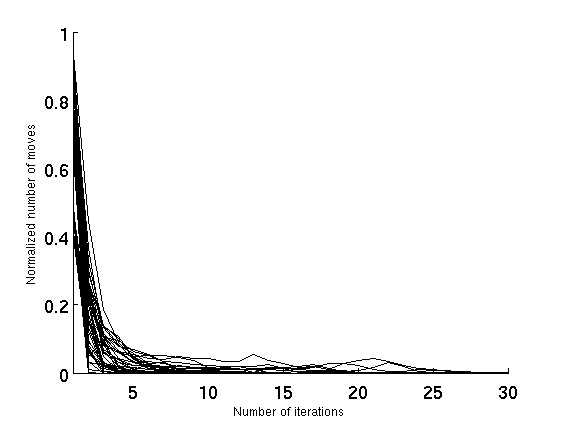
\includegraphics[scale=0.6]{figures/iterMove.png} 
\caption{Number of moved objects per iteration when clustering a variety of datasets with the k-averages algorithm, normalized by the total number of objects to cluster. The datasets used to create this figure are the real-life time series data that we employ for experimental validation, \textit{cf.} Section~\ref{sec:experiments}.}
\label{fig:moved}
\end{figure}

To go further in this analysis, we propose with Figure~\ref{fig:totalMoved} to consider the total number of object reallocation over a full run of the kaverages algorithms. As can be seen, the correlation is clearly linear with the number of objects to cluster. In fact, the number of reallocations is roughly equal to the number of objects to cluster, which allows us to reach for k-averages a (statistical) total complexity of $O(n^2)$ instead of $O(n^2)$ per iteration.

\begin{figure}
\center
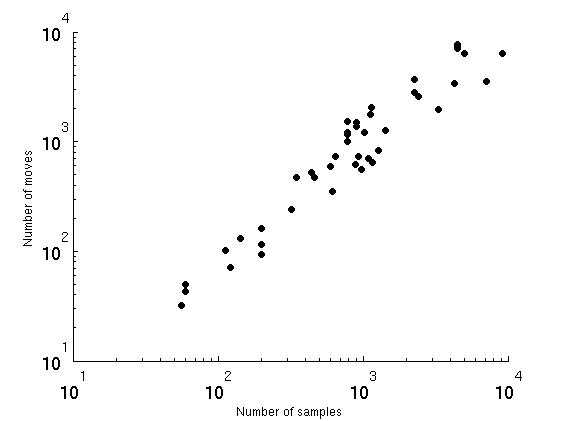
\includegraphics[scale=0.6]{figures/sampleMove.png} 
\caption{Total number of object reallocations over a run of the kaverages algorithm, plotted against the number of objects to be clustered. The datasets used to create this figure are the real-life time series data that we employ for experimental validation, \textit{cf.} Section~\ref{sec:experiments}.}
\label{fig:totalMoved}
\end{figure}

\subsection{Memory access}

The lowered computational costs is also accompanied by a decrease in memory access: as can be seen from Equation~\ref{eq:newSimilNewC}, in order to compute the new object-to-class similarities after moving an object $n$, only line $n$ of the similarity matrix needs to be read. For the rest of the algorithm, only the (much smaller) object-to-class similarity matrix is used. By contrast, in the case of kernel k-means, the computation of $M_c$ values at each iteration require that the whole similarity matrix be read, which can be a serious performance bottleneck in the case of large object collections.

Moreover, the similarity update function of k-averages, by reading one line of the matrix at a time, presents good data locality properties, which make it play well with standard memory paging strategies.

To illustrate and confirm the theoretical complexity computed here, the next section proposes some performance figures measured on controlled datasets.

\section{Validation}
\label{sec:validation}

In order to reliably compare the clustering quality and execution speed between the two approaches, we have written simple C implementations of Algorithms~\ref{algo:kkmeans_optim} and~\ref{algo:kaverages}, with minimal operational overhead: both read the similarity matrix from a binary file where all matrix values are stored sequentially in standard reading order, line by line, and write out the result of the clustering as a label text file. Both implementations use reasonably efficient code, but without advanced optimizations or parallel processing. All code can be found at <online reference>.

The figures presented in this section were obtained on simple synthetic datasets, in order to give precise control on the features of the analyzed data: for $n$ points split between $C$ classes, $C$ centroids are generated at random in 2D space, each point is given a random class, and point coordinates are generated following a Gaussian distribution around class centroids. In addition to numbers of objects and classes, the variance of Gaussian distributions can be adjusted to modulate how clearly separable clusters are. Similarities are computed as inverse Euclidean distances between points. This clearly simplified example is useful as a first control test bench; the next section is dedicated to experiments on more realistic datasets.

\subsection{Clustering performance}

Several metrics are available to evaluate the performance of a clustering algorithm. The one closest to the actual target application is the raw accuracy, that is the average number of items labeled correctly after an alignment phase of the estimated labeling with the reference one (\cite{Kuhn1955Hungarian}).

Another metric of choice, is the Normalized Mutual Information (NMI) criterion. Based on information theoretic principles, it measures the amount of statistical information shared by the random variables representing the predicted cluster distribution and the reference class distribution of the data points. If $P$ is the random variable denoting the cluster assignments of the points, and $C$ is the random variable denoting the underlying class labels on the points then the NMI measure is defined as:
\begin{equation}
\textbf{NMI} = \frac{ 2\- I(C;K) }{H(C)+H(K)}
\end{equation}

where $I(X;Y)=H(X)−H(X|Y)$ is the mutual information between the random variables $X$ and $Y$, $H(X)$ is the Shannon entropy of $X$,and $H(X|Y)$ is the conditional entropy of $X$ given $Y$. Thanks to the normalization, the metric stays between $0$ and $1$, $1$ indicating a perfect match, and can be used to compare clustering with different numbers of clusters. Interestingly, random prediction gives an NMI close to $0$, whereas the accuracy of a random prediction on a balanced bi-class problem is as high as 50\,\%.

For those reasons and ease of reading, only the NMI is considered here, as in (\cite{Kulis2008}). However, it shall be noted that most of the statements that will be made in the following in terms of ranking of the different algorithms  still holds true while considering the accuracy metric as reference.

\begin{figure}
\center
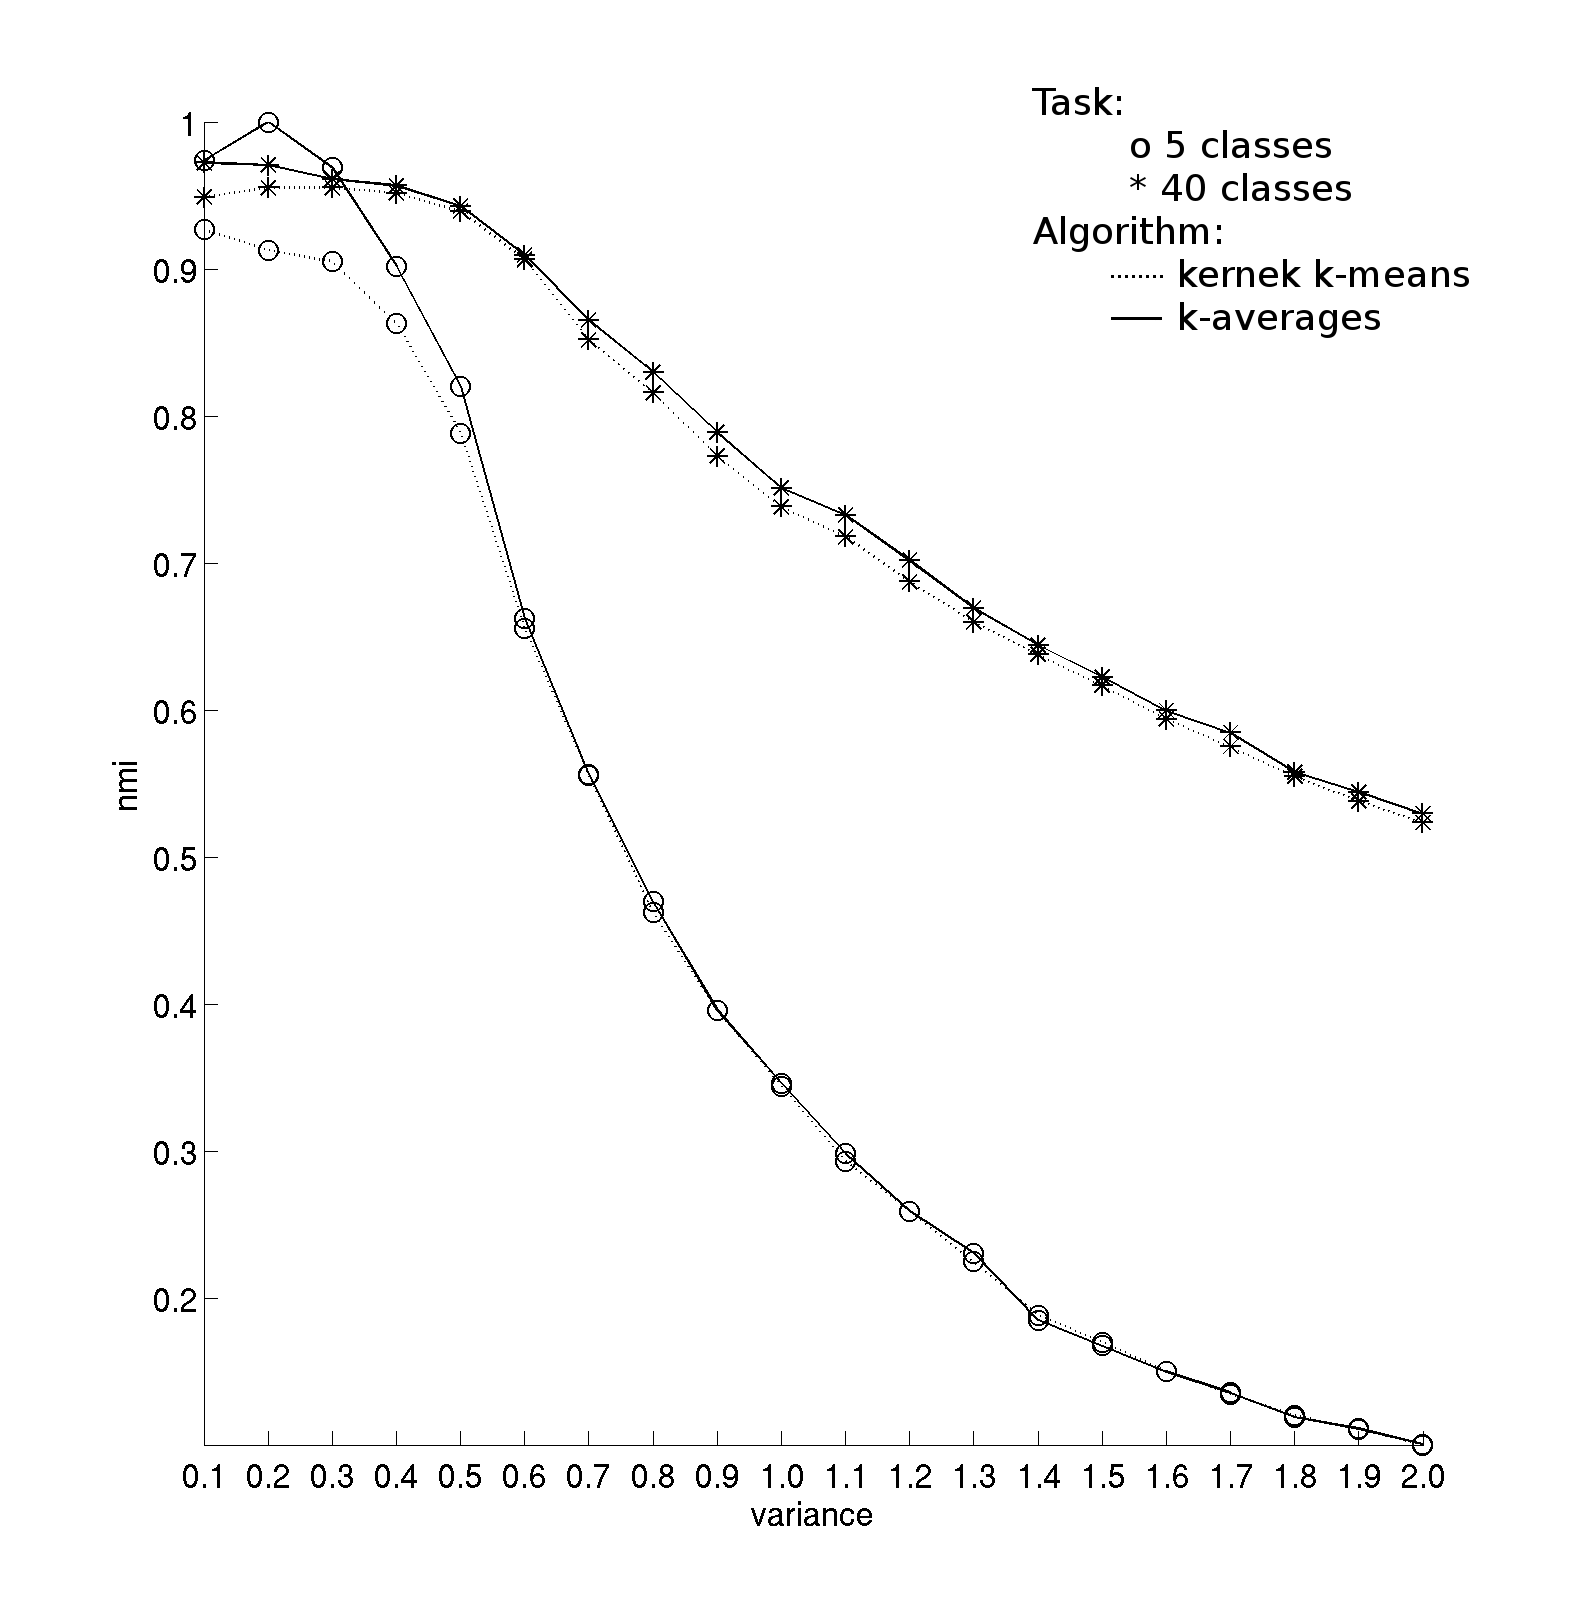
\includegraphics[scale=0.4]{figures/synthetic.png} 
\caption{NMI of kernel k-means and k-averages clustering relative to ground truth for synthetic data sets of 5 and 40 classes, as a function of the \gl{spread} of those classes (and hence, their degree of overlap). The lower values of NMI for 5-class experiments is in fact an artifact introduced by the normalization, and is not significant here; we only focus, for each series of experiments, on the relative performances of kernel k-means and k-averages.}
\label{fig:synth_perf}
\end{figure}

Figure~\ref{fig:synth_perf} presents the quality of clusterings obtained using kernel k-means (dotted line) and k-averages (solid line) on two series of datasets: one featuring 5 classes, the other 40 classes. On the x-axis is the variance of the Gaussian distribution used to generate point cloud for each class: the higher that value, the more the classes are spread out and overlap each other, thus making the clustering harder.

The question of choosing the proper number of clusters for a given dataset without \textit{a priori} is a well known and hard problem, and well beyond the scope of this article. Therefore, for the purpose of evaluation, clustering is done by requesting a number of clusters equal to the actual number of classes in the dataset. In order to obtain stable and reliable figures, clustering is repeated 500 times with varying initial conditions, \textit{i.e.} the initial assignment of points to clusters is randomly determined, and only the average performance is given. For fairness of comparison, each algorithm is run with the exact same initial assignments.

As can be seen on the figure, in the case of a 5-class problem, k-averages outperforms kernel k-means in the \gl{easy} cases (low class spread), before converging to equivalent results. For the more complex 40-class datasets, k-averages consistently yields a better result than kernel k-means, especially for higher values of the variance.

\subsection{Time efficiency}

Figure~\ref{fig:timing} shows the average time spent by kernel k-means and k-averages to cluster synthetic datasets or varying sizes. As previously, initial conditions on each run are identical for both algorithms.

\begin{figure}
\center
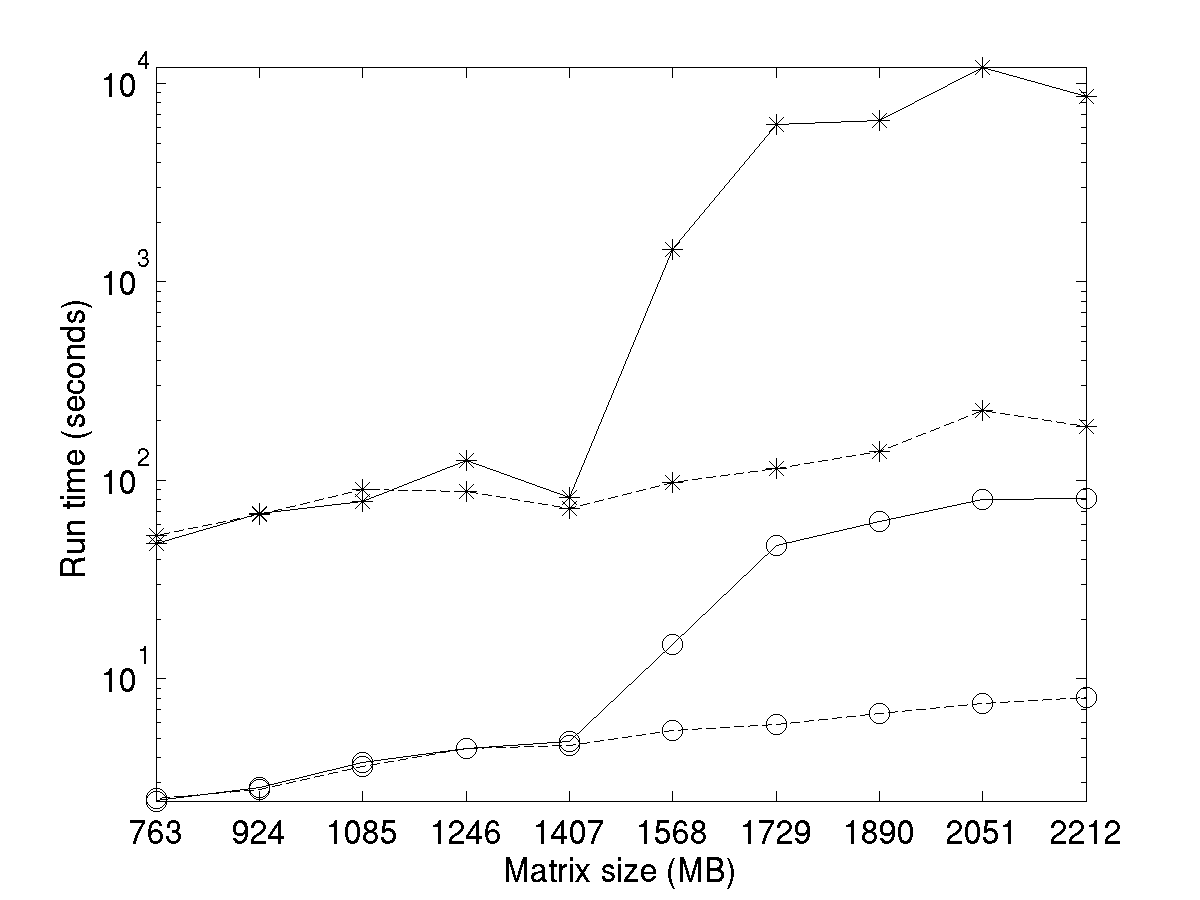
\includegraphics[scale=0.4]{figures/simpleSwap.png} 
\caption{Average computation time of the kernel k-means (*) and kaverages (o) algorithms on computers with 2 GB (solid line) and 32 GB (dashed line) of RAM, respectively. The \gl{running time} axis follows a logarithmic scale.}
\label{fig:timing}
\end{figure}

These figures confirm the theoretical complexity analysis presented in Section~\ref{sec:complexity}: k-averages runs at least 20 times faster on average than kernel k-means in ordinary conditions, when  available memory is not an issue. When the matrix size exceeds what can be stored in RAM and the system has to resort to paged memory, as in the presented experiments when the matrix reaches about 1500MB, both algorithms suffer from a clear performance hit; however, kernel k-means is much more affected, and the difference becomes even more significant: with a 2000MB similarity matrix on a memory-limited computer, k-averages runs about 100 times faster than kernel k-means.

Having established the interest of our proposed method relative to kernel k-means on synthetic object collections, we now proceed to a thorough evaluation on real-life data.

\section{Experiments}
\label{sec:experiments}

In order to demonstrate the usefulness of k-averages when dealing with real data, we have chosen to focus on the clustering of times series as the evaluation task.

Time series, even though represented as vectors and therefore suitable for any kinds of norm-based clustering, are best compared with elastic measures (\cite{Ding:2008:QMT:1454159.1454226, Wang:2013:ECR:2429736.2429754}), due to their varying length. The Dynamic Time Warping (DTW) measure is an elastic measure widely used in many areas since its introduction for spoken word detection \cite{1163055} and has never been significantly challenged for time series mining (\cite{conf/kdd/BerndtC94, Rakthanmanon:2013:ABD:2513092.2500489}).

Effective clustering of time series using the DTW measure require similarity based algorithms such as the k-average algorithm. With some care, kernel based algorithm can also be considered provided that the resulting similarity matrix is converted into a kernel, \textit{i.e.} the matrix is forced to be semi definite positive to be a Gram matrix (\cite{Lanckriet:2004:LKM:1005332.1005334}).

In order to demonstrate the superior relevance for this type of data of a similarity-based clustering making use of the DTW measure, compared with a simple Euclidean distance method, we shall give as reference in the following tables the results of a simple k-means clustering.

\subsection{Datasets}

To compare quality of clusterings obtained by the considered algorithms, we consider a large collection of 43 time series datasets created by many laboratories all over the world and compiled by Prof. Keogh (\url{www.cs.ucr.edu/~eamonn/time_series_data}).  Statistics about the morphology of those datasets are summarized in Table~\ref{tab:dbs}.

\begin{table}
\center
\begin{tabular}{l|ccc}
& min & average $\pm$ variance & max \\
\hline
number of classes & 2 & 8 $\pm$ 9 & 50 \\
number of time series & 56 & 1626 $\pm$ 2023 & 9236 \\
time series length & 24 & 372 $\pm$ 400 & 1882 \\
\end{tabular}
\caption{\label{tab:dbs} Statistics of the datasets. The length of the times series is expressed in samples.}
\end{table}

\subsection{Evaluation Protocol}

For each dataset, since we perform clustering, and not supervised learning, the training and testing data are joined. If relevant, the DTW is computed using the implementation provided by Prof. Ellis (\url{http://www.ee.columbia.edu/~dpwe/resources/matlab/dtw}) with default parameters.

As in our previous experiments with synthetic data, we choose here the normalized mutual information as measure of clustering quality; clustering is done by requesting a number of clusters equal to the actual number of classes in the dataset, and repeated 500 times with varying initial conditions, each algorithm being run with the exact same initial assignments.

\subsection{Results}

For ease of readability and comparison, the presented results are split into 3 tables. Table~\ref{tab:results-2} lists the results obtained on bi-class datasets, \textit{i.e.} the datasets annotated in terms of presence or absence of a given property; Table~\ref{tab:results-37} concerns the datasets with a small number of classes (from 3 to 7); and Table~\ref{tab:results-8} focuses the datasets with a larger number of classes (from 8 to 50).

For each experiment, the result of the best performing method is marked by a star, and results equivalent to the best are highlighted in bold. It should be noted that this decision is the result of a statistical analysis on the 500 runs performed; it can therefore happen, without contradiction, that a method has a higher average NMI than the other but is not significantly better, or, conversely, that it does perform significantly better despite an identical average NMI.

%% BI-CLASS

\begin{table} 
\begin{center} 
\small 
 \setlength{\tabcolsep}{1em}
 \renewcommand{\arraystretch}{1.2}
\begin{tabular}{lccccc} 
id & classes & objects & k-means & kernel k-means & k-averages \\ 
&  &  & (NMI $\times 0.01$) & (NMI $\times 0.01$) & (NMI $\times 0.01$) \\ 
\hline 
 7 & 2 &   56 & 5$\pm$1 & \textbf{6$\pm$3$^*$} & 5$\pm$1 \\ 
12 & 2 &  200 & 12$\pm$2 & 14$\pm$2 & \textbf{15$\pm$1$^*$} \\ 
13 & 2 &  884 & 0$\pm$0 & \textbf{3$\pm$2$^*$} & \textbf{3$\pm$2} \\ 
17 & 2 &  200 & \textbf{0$^*$} & \textbf{0$^*$} & \textbf{0$^*$} \\ 
20 & 2 & 1096 & 0$\pm$0 & \textbf{1$\pm$0$^*$} & 1$\pm$0 \\ 
21 & 2 &  121 & \textbf{3$\pm$1$^*$} & 1$\pm$1 & 1$\pm$0 \\ 
25 & 2 & 1272 & 30$\pm$0 & 52$\pm$0 & \textbf{53$\pm$0$^*$} \\ 
28 & 2 &  621 & 51$\pm$25 &  78$\pm$0 & \textbf{ 78$\pm$0$^*$} \\ 
29 & 2 &  980 & \textbf{24$^*$} & 21 & 21 \\ 
34 & 2 & 1162 & 0$\pm$0 & \textbf{7$\pm$0$^*$} & 7$\pm$0 \\ 
42 & 2 & 7164 & \textbf{0$^*$} & 0 & 0 \\ 
43 & 2 & 3300 & 0$\pm$0 & \textbf{0$\pm$0} & \textbf{0$\pm$0$^*$} \\ 
\hline 
 &  & count & 4 & 6 & 6 \\ 
\end{tabular} 
\end{center} 
\caption{Average NMI of clusterings by k-means, kernel k-means and k-averages for bi-class datasets over 500 runs of the algorithms. The last row gives for each method the number of datasets where it performs best.}
\label{tab:results-2} 
\end{table} 
 
 %% 3-7 classes
 
   
\begin{table} 
\begin{center} 
\small 
 \setlength{\tabcolsep}{1em}
 \renewcommand{\arraystretch}{1.2}
\begin{tabular}{lccccc} 
id & classes & objects & k-means & kernel k-means & k-averages \\ 
&  &  & (NMI $\times 0.01$) & (NMI $\times 0.01$) & (NMI $\times 0.01$) \\ 
\hline 
 3 & 5 &   60 & \textbf{38$\pm$2$^*$} & 35$\pm$3 & 35$\pm$2 \\ 
 4 & 3 &  930 & 36$\pm$1 & \textbf{51$\pm$4} & \textbf{51$\pm$3$^*$} \\ 
 5 & 3 & 4307 & 0$\pm$0 & \textbf{0$\pm$0$^*$} & 0$\pm$0 \\ 
 6 & 4 & 1420 & 24$\pm$3 & 43$\pm$5 & \textbf{44$\pm$4$^*$} \\ 
11 & 4 &  322 &  82$\pm$5 & 83$\pm$10 & \textbf{ 89$\pm$8$^*$} \\ 
15 & 4 &  112 & 44$\pm$4 & \textbf{66$\pm$8$^*$} & 65$\pm$7 \\ 
18 & 5 &  463 & 9$\pm$0 & \textbf{9$\pm$1$^*$} & \textbf{9$\pm$0} \\ 
19 & 7 &  650 & \textbf{5$\pm$1} & \textbf{5$\pm$1$^*$} & \textbf{5$\pm$1} \\ 
22 & 7 &  143 & 44$\pm$2 & 51$\pm$3 & \textbf{52$\pm$1$^*$} \\ 
26 & 6 &  442 & 22$\pm$2 & 22$\pm$3 & \textbf{23$\pm$3$^*$} \\ 
27 & 4 &   60 & \textbf{54$\pm$5$^*$} & 46$\pm$8 & 50$\pm$7 \\ 
30 & 3 & 9236 & 60$\pm$0 & \textbf{61$\pm$2$^*$} & 60$\pm$0 \\ 
32 & 6 & 1020 & 76$\pm$5 & \textbf{80$\pm$4$^*$} & \textbf{80$\pm$1} \\ 
33 & 4 &  200 & 52$\pm$2 & \textbf{57$\pm$6$^*$} & 53$\pm$3 \\ 
35 & 4 & 5000 &   2$\pm$0 & \textbf{15$\pm$11$^*$} & 14$\pm$12 \\ 
37 & 7 &  350 & 31$\pm$2 & 42$\pm$2 & \textbf{42$\pm$1$^*$} \\ 
38 & 6 &  600 & 79$\pm$3 & 84$\pm$4 & \textbf{88$\pm$3$^*$} \\ 
\hline 
 &  & count & 3 & 9 & 10 \\ 
\end{tabular} 
\end{center} 
\caption{Average NMI of clusterings by k-means, kernel k-means and k-averages for datasets of 3 to 7 classes, over 500 runs of the algorithms. The last row gives for each method the number of datasets where it performs best.}
\label{tab:results-37}
\end{table} 
 
 
 %% 8-50 classes
 
   
\begin{table} 
\begin{center} 
\small 
 \setlength{\tabcolsep}{1em}
 \renewcommand{\arraystretch}{1.2}
\begin{tabular}{lccccc} 
id & classes & objects & k-means & kernel k-means & k-averages \\ 
&  &  & (NMI $\times 0.01$) & (NMI $\times 0.01$) & (NMI $\times 0.01$) \\ 
\hline 
 1 & 50 &  905 & 64$\pm$1 & 70$\pm$1 & \textbf{72$\pm$1$^*$} \\ 
 2 & 37 &  781 & 58$\pm$1 & 63$\pm$1 & \textbf{66$\pm$1$^*$} \\ 
 8 & 12 &  780 & 26$\pm$1 & 26$\pm$2 & \textbf{27$\pm$1$^*$} \\ 
 9 & 12 &  780 & 33$\pm$2 & 33$\pm$2 & \textbf{33$\pm$1$^*$} \\ 
10 & 12 &  780 & 27$\pm$1 & 26$\pm$2 & \textbf{27$\pm$1$^*$} \\ 
14 & 14 & 2250 & 37$\pm$2 & \textbf{78$\pm$2$^*$} & 75$\pm$2 \\ 
16 & 14 & 2250 & 37$\pm$2 & 78$\pm$2 & \textbf{79$\pm$2$^*$} \\ 
23 &  8 & 2400 & 87$\pm$4 & 89$\pm$4 & \textbf{90$\pm$3$^*$} \\ 
24 & 10 & 1141 & 25$\pm$1 & 31$\pm$2 & \textbf{32$\pm$1$^*$} \\ 
31 & 15 & 1125 & 54$\pm$1 & 66$\pm$2 & \textbf{68$\pm$1$^*$} \\ 
36 & 25 &  905 & 43$\pm$1 & 51$\pm$1 & \textbf{52$\pm$1$^*$} \\ 
39 &  8 & 4478 & 44$\pm$1 & 46$\pm$1 & \textbf{46$\pm$1$^*$} \\ 
40 &  8 & 4478 & 44$\pm$0 & 45$\pm$0 & \textbf{45$\pm$0$^*$} \\ 
41 &  8 & 4478 & 42$\pm$1 & \textbf{43$\pm$0$^*$} & 43$\pm$0 \\ 
\hline 
 &  & count & 0 & 2 & 12 \\ 
\end{tabular} 
\end{center} 
\caption{Average NMI of clusterings by k-means, kernel k-means and k-averages for datasets of 8 to 50 classes, over 500 runs of the algorithms. The last row gives for each method the number of datasets where it performs best.}
\label{tab:results-8}
\end{table} 
 
A first obvious conclusion of the presented data is that, while k-means can occasionally outperform the more advanced methods, especially in the case of bi-class problems, its results are overall, as expected, clearly inferior to those of a similarity-based clustering using the DTW measure. We shall therefore focus on the difference between kernel k-means and k-averages.

Setting aside simple k-means, k-averages yields the best clustering for 26 datasets out of 43, while kernel k-means takes the lead in 14 cases, the three remaining ones being equivalent. Considering results more closely, one can see that k-averages is equivalent to kernel k-means for bi-class problems, slightly better for moderate numbers of classes, and yields clearly better results (12 out of 14) for datasets featuring more than 8 classes. This is remarkably consistent with the observations made in Section~\ref{sec:validation} on synthetic data.

\section{Conclusion}

We have presented k-averages, an iterative flat clustering algorithm that operates on arbitrary similarity matrices by explicitly and directly aiming to optimize the average intra-class similarity. Having established the mathematical foundation of our proposal, including guaranteed convergence, we have thoroughly compared it with the widely used standard method, kernel k-means, showing that our algorithm converges much faster (20 times faster under ordinary conditions) and to slightly better results, while also being more sparing in memory use.

A particularly interesting result is that k-averages seems to yield clearly better results than kernel k-means in the case of problems with many classes (8 and more); this is confirmed both on synthetic test data and on real-life data.

Implementations of k-averages in Matlab and C are freely available as mature code ready for general use, at <url>. That repository also contains the reference C implementation of kernel k-means which we have used for the experiments reported in this article.

\bibliography{bib}

\end{document}
